%------------------------------------------------------------
% Description : Calculus in \R^n space
% Author      : taxus-d <iliya.t@mail.ru>
% Created at  : ??? 
%------------------------------------------------------------
\documentclass[12pt,trimbord]{../../../notes}
\usepackage{silence}
\WarningFilter{latex}{Reference}
\graphicspath{{../../img/}}

\begin{document}

\paragraph{Оценка приращения дифференциального отображения}
\label{par:diffspace::diffestim}

\begin{prop}\label{prop:diffspace::diffestim::lagrfail}
  Пусть $f\colon \R^n \to \R^m$, $m \geqslant 2$. Тогда формула Лагранжа
  \[
    f(b) - f(a) = f'(c)(b - a)
  \]
  не работает.
\end{prop}
\begin{exmp*}\label{exmp:diffspace::diffestim::lagrfail}
  Пусть 
  \[
    f(t) := (\cos t, \sin t), b - a = 2\pi
  \]
\end{exmp*}

\begin{thrm}[об оценке приращения отображения]\label{thrm:diffspace::diffestim::diffestim}
  Пусть $f\colon G \subset \R^n \to \R^m$, $G$~--- выпуклое, $f$~--- дифференцируема, 
  \[ 
    \forall\, x \in G \;\: \| f'(x) \| \leqslant M 
  \]
  Тогда $\forall\, a,b \in G \;\: \|f(b) - f(a)\| \leqslant M \| b-a \|$
\end{thrm}

\begin{ittproof}
  <<Окружим>>  исходную функцию:
  \[
    F = \psi \circ f \circ \varphi
  \]
  где 
  \begin{align*}
    \varphi&: \R^n \to \R^m & \varphi(t) &:= t(b-a) + a, & t&\in [0,1] \\
    \psi&: \R^m \to \R & \psi(y) &:= \langle y, \ell \rangle, & \ell &= f(b)-f(a) 
  \end{align*}
  Заметим, что $F$~--- обычная вещественнозначная функция. Так что для неё работает формула
  Лагранжа:
  \[
    \exists\, c \in [0,1] \colon F(1)-F(0) = F'(c)(1-0) = F'(c)
  \]
  Тогда из свойств нормы (по ходу дела обозначим $\varphi(c)$ за $x$):
  \[
    \|F'(c)\| = \|\psi'(f(x)) \cdot f'(x) \cdot \varphi'(c)\| \leqslant 
    \|\psi'(f(x)) \| \cdot \| f'(x) \| \cdot \| \varphi'(c)\|
  \]
  Здесь тонкость в обозначениях. Производные~--- вроде матрицы, поэтому их нормы~--- что-то
  странное на первый взгляд. На самом деле смысл немного иной. 
  \[
    \mathrm d L(x, h) = f'(x) \cdot h
  \]
  Таким образом, дифференциал~--- неплохое линейное отображение. А под <<нормой производной>>
  имеется в виду норма соответствующего линейного отображения.

  Теперь давайте что-нибудь скажем про эти нормы. 
  \begin{enumerate}
    \item $\varphi'(t) = (b-a) \Rightarrow \| \varphi'(c) \| = \| b - a\|$
    \item $\psi(y) = \langle y, l \rangle$, $\| \psi\| = \|\ell\|$      
  \end{enumerate}
  Так что 
  \[
    \| F'(c)\| \leqslant M \cdot \| \ell \| \cdot \|b-a\|
  \]
  С другой стороны:
  \[
    F(1) - F(0) = \psi(f(b)) - \psi(f(a)) = \langle f(b), \ell \rangle - \langle f(a), \ell \rangle
    = \langle \ell, \ell \rangle  = \|\ell \|^2
  \]
  В итоге, совмещая оба выражения, приходим к утверждению теоремы.
\end{ittproof}

\paragraph{Частные производные высших порядков}
\label{par:diffspace::highpartial}

\begin{defn}\label{defn:diffspace::highpartial}
  Пусть $f \colon G \subset \R^n \to \R$, существуют производные $k$-го порядка. Тогда
  \[
    \partial_{i_1, \dotsc, i_{k+1}}^{k+1} f(x) := \partial_{i_{k+1}}(\partial^k_{i_1, \dotsc, i_{k+1}} f) (x)
  \]
\end{defn}
\begin{rem}\label{rem:diffspace::highpartial::smooth}
  $C^p(G)$~--- класс функций, определённых в $G$ с непрерывной производной до $p$-го порядка
  включительно.
  Функции из $C^1$ ещё называются гладкими.
\end{rem}

\begin{thrm}[Зависимость производных $p$-го порядка от перестановки переменных]
  \label{thrm:diffspace::highpartial::permut}
  Пусть \mbox{$f \in C^p(G)$}, $x\in G$. При этом
  \[
    \begin{split}
      i &= \{ i_1, \dotsc, i_p \mid i_k \in \{1, \dotsc, n\}\} \\
      j &= \{ j_1, \dotsc, j_p \mid j_k \in \{1, \dotsc, n\}\} \\
      j &= \pi(i)
    \end{split}
  \]
  Тогда 
  $\partial_i^{\,p} f(x) = \partial_j^{\,p} f(x)$
\end{thrm}
\begin{rem}\label{rem:diffspace::highpartial::permut}
  Тут важно, что есть целая окрестность. Одной точки не хватит.
\end{rem}

\paragraph{<<Многомерный>> дифференциал высоких порядков}
\label{par:diffspace::highdiff}

\begin{defn}\label{defn:diffspace::highdiff}
  Пусть $f \colon G \subset \R^n \to \R$, $f\in C^p(G)$
  \[  
    \del^p f(x) := \sum_{1 \leqslant i_1 \leqslant \dotsb \leqslant i_p \leqslant n}
    \frac{\partial^p f}{\partial x_{i_p} \dotso \partial x_{i_p}} \, \del x_{i_1} \dotsm \del x_{i_p}
  \]
\end{defn}

\begin{stat}\label{stat:diffspace::highdiff::binom}
  Если частные производные можно переставлять, то
  \[
    \del^p f(x) = \sum_{\substack{\alpha_i \geqslant 0 \\ \sum \alpha_i = p}} 
    \frac{p!}{\alpha_1! \dotsm \alpha_n!} \, 
    \frac{\partial^p f}{\partial x_1^{\alpha_1}\dotso \partial x_n} \,\del x_{i_1} \dotsm \del x_{i_p}
  \]
\end{stat}

\paragraph{Формула Тейлора для функций многих переменных}
\label{par:diffspace::taylor}

\begin{thrm}\label{thrm:diffspace::taylor}
  Пусть $f \in C^p(G), G\in \R^n$, $a\in G$. Пусть также $h\in \R^n \colon a+h \in G$.
  Тогда 
  \[
    f(a+h) = \sum_{k=0}^p \frac{1}{k!} \, \del^k f(a,h) + R_p(h)
  \]
  Остаток $R_p(h)$ можно представить несколькими способами:
  \begin{enumerate}
    \item В форме Пеано: $R_p(h) = o(\|h\|^p)$
    \item В форме Лагранжа: $R_p(h) = \dfrac{1}{(p+1)!}\, \del^{p+1} f(a + \theta h, h)$, 
      $\theta \in (0,1)$
  \end{enumerate}

\end{thrm}

\paragraph{Экстремумы}
\label{par:diffspace::extrema}

\begin{defn}\label{defn:diffspace::extrema}
  Пусть $f\colon G \subset \R^n \to \R$, $a\in G$. Тогда говорят, что $f$ имеет в $a$ максимум (нестрогий), если
  \[
    \exists\, U(a) \colon \forall\, x \in U \;\: f(x) \leqslant f(a)
  \]
  Когда неравенство строгое, а окрестность проколотая, то максимум~--- строгий
  Для минимума нужно $\geqslant$.
\end{defn}

\begin{thrm}[Необходимое условие экстремума]\label{thrm:diffspace::extrema::ness}
  Пусть $a$ внутренняя точка $G \subset \R^n$, $f\in C^1(a)$. Тогда если $f$ имеет в $a$ экстремум, то
  \[
    \del f(a) = 0 \Leftrightarrow \forall\,i \;\: \partial_i f(a) = 0
  \]
\end{thrm}

\begin{thrm}[Необходимое условие экстремума]\label{thrm:diffspace::extrema::suff}
  Пусть $a\in G \subset \R^n$, $a$~--- внутренняя точка, $f\in C^2(a)$.
  \begin{enumerate}
    \item $\del f(a) = 0$, $\del^2 f(a) > 0 \Rightarrow$ $f$ имеет в $a$ $\min$
    \item $\del f(a) = 0$, $\del^2 f(a) < 0 \Rightarrow$ $f$ имеет в $a$ $\max$
    \item $\del f(a) = 0$, $\del^2 f(a) \lessgtr 0 \Rightarrow$ ничего нет
    \item $\del f(a) = 0$, $\del^2 f(a) \leqslant 0 \Rightarrow$ $f$ не имеет в $a$ $\min$
    \item $\del f(a) = 0$, $\del^2 f(a) \geqslant 0 \Rightarrow$ $f$ не имеет в $a$ $\max$
  \end{enumerate}
\end{thrm}

\paragraph{Понятие о неявной функции}
\label{par:diffspace::implicit2}

\begin{defn}\label{defn:diffspace::implicit2}
  Пусть $F\colon G \subset \R^2 \to \R$. Рассмотрим уравнение
  \begin{equation}
    \label{eq:diffspace::implicit2::base}
    F(x, y) = 0
  \end{equation}

  Пусть $a =(x_0, y_0)$ удовлетворяет \ref{eq:diffspace::implicit2::base}, 
  а $U$~--- окрестность $a \colon$ $U = U_x \times U_y$.
  Тогда будем говорить, что уравнение \ref{eq:diffspace::implicit2::base} определяет неявную 
  функцию $f$ в $U$, если
  \[
    \forall\, x\in P \; \exists!\, y\in Q \colon F(x,y) = 0 \hspace{1.5em} (y = f(x))
  \]
\end{defn}

\begin{thrm}[О неявной функции]\label{thrm:diffspace::implicit2}
  Пусть $F\colon G\subset \R^2 \to \R$, $F\in C^1(x_0,y_0)$, а $a=(x_0, y_0) \colon$
  \begin{enumerate}
    \item $F(x_0, y_0) = 0$
    \item $F_y'(x_0, y_0) \neq 0$
  \end{enumerate}
  Тогда 
  $\exists\, P(x_0), Q(y_0) \colon $ в $U = P\times Q$ уравнение \ref{eq:diffspace::implicit2::base} 
  задаёт неявную функцию $f\colon P\to Q$. При этом
  \[
    f\in C^1 \land f'(x) = - \frac{F_x'(x,y)}{F_y'(x,y)}
  \]
\end{thrm}
\begin{ittproof}
  \begin{enumerate}
    \item (Доказательство существования) \\
      Рассмотрим $\varphi(y) = F(x_0, y)$. Пусть НУО $F_y'(x_0, y_0) > 0$.
      Тогда 
      \[
        \exists\, U_\varepsilon(x_0, y_0) \colon \forall\, x, y \in U \;\: F_y'(x, y) > 0
      \]
      Обозначим соответствующие проекции $U$ (шар) на координатные оси за $U_x, U_y$
      Получается, что $\varphi \uparrow U_y = (y_0 - \varepsilon; y_0 + \varepsilon)$.
      Тогда 
      \[
        \begin{split}
          \exists\, V_1(x_0) &\colon \forall\, x\in V_1 F(x, y+\varepsilon) > 0 \\
          \exists\, V_2(x_0) &\colon \forall\, x\in V_2 F(x, y-\varepsilon) < 0 \\
                           P &= V_1 \cap V_2
        \end{split}
      \]
      Тогда из теоремы Больцано-Коши и монотонности $\varphi$
      \[
        \forall\, x \in P \; \exists!\, y\in Q=U_y \colon F(x, y) = 0
      \]
      В итоге получилось определение неявной функции.
    \item Непрерывность в $(x_0, y_0)$ вроде очевидна, мы же каждому $x$ из $P$ сопоставили 1
      $y$ из $Q$. Принадлежность классу $C$ можно установить проведя аналогичные рассуждения
      для $x\in P(x_0)$
    \item С гладкостью что-то странное. Можно наверное сделать как в Зориче.
    \item $F(x, f(x)) \equiv 0 \Rightarrow F_x'\cdot 1 + F_2'f'(x) = 0$
  \end{enumerate}
\end{ittproof}

\paragraph{Полнота пространства \texorpdfstring{$\R^n$}{}}
\label{par:diffspace::banach}

\paragraph{Теорема о сжимающем отображении}
\label{par:diffspace::contrmap}

\begin{defn}\label{defn:diffspace::contrmap}
  Пусть $(X, \rho)$~--- метрическое пространство. Тогда отображение $T\colon X \to X$ называется
  сжимающим, если 
  \[
    \exists\, C \in (0,1) \colon \forall\, x',x'' \rho(T(x'), T(x'')) 
    \leqslant C\cdot \rho(x',x'')
  \]
\end{defn}

\begin{thrm}[Банах]\label{thrm:diffspace::contrmap::banach}
  Пусть $(X, \rho)$~--- полное метрическое пространство, а отображение $T\colon X \to X$~--- сжимающее.
  Тогда $\exists!\, x_* \in X \colon Tx_* = x_*$ (неподвижная точка).

  Ещё часто ссылаются на следующий факт, появляющийся в процессе доказательства:
  \[
    \forall\, x_0 \in X \; \exists\, \lim_{n\to \infty} T^n x_0 = x_*
  \]
\end{thrm}

\paragraph{Метод Ньютона}
\label{par:diffspace::newtfindroot}
потом

\paragraph{Теорема об обратном отображении(формулировка)}
\label{par:diffspace::invmaphandwave}

Пусть $F: G\subset \R^n \to \R^m$~--- гладкое. Порассуждаем, когда может существовать $F^{-1}$.

\rule{\textwidth}{0.5pt}

Рассмотрим, например, линейное отображение.
\[
  y = F(x) = Ax \Leftrightarrow 
  \begin{cases}
    y_1 = a_{11} x_1 + \dotsb + a_{1n} x_n \\
    \hdotsfor{1}\\
    y_m = a_{m1} x_1 + \dotsb + a_{mn} x_n
  \end{cases}
\]

Понятно, что в таком случае задача поиска обратного отображения сводится к поиску обратной матрицы.
Тогда из линала ясно, что для того, чтобы у нас всё вышло, нужно
\[
  m = n \land \det A \neq 0 
\]

\rule{\textwidth}{0.5pt}

Теперь попытаемся обобщить на остальные функции. 

Пусть $a\in G$, $b = F(a)$
\[
  (?) \exists\, U(a), V(b) \,\colon \: F\colon U \leftrightarrow V
\]

\begin{figure}[h]
  \centering
  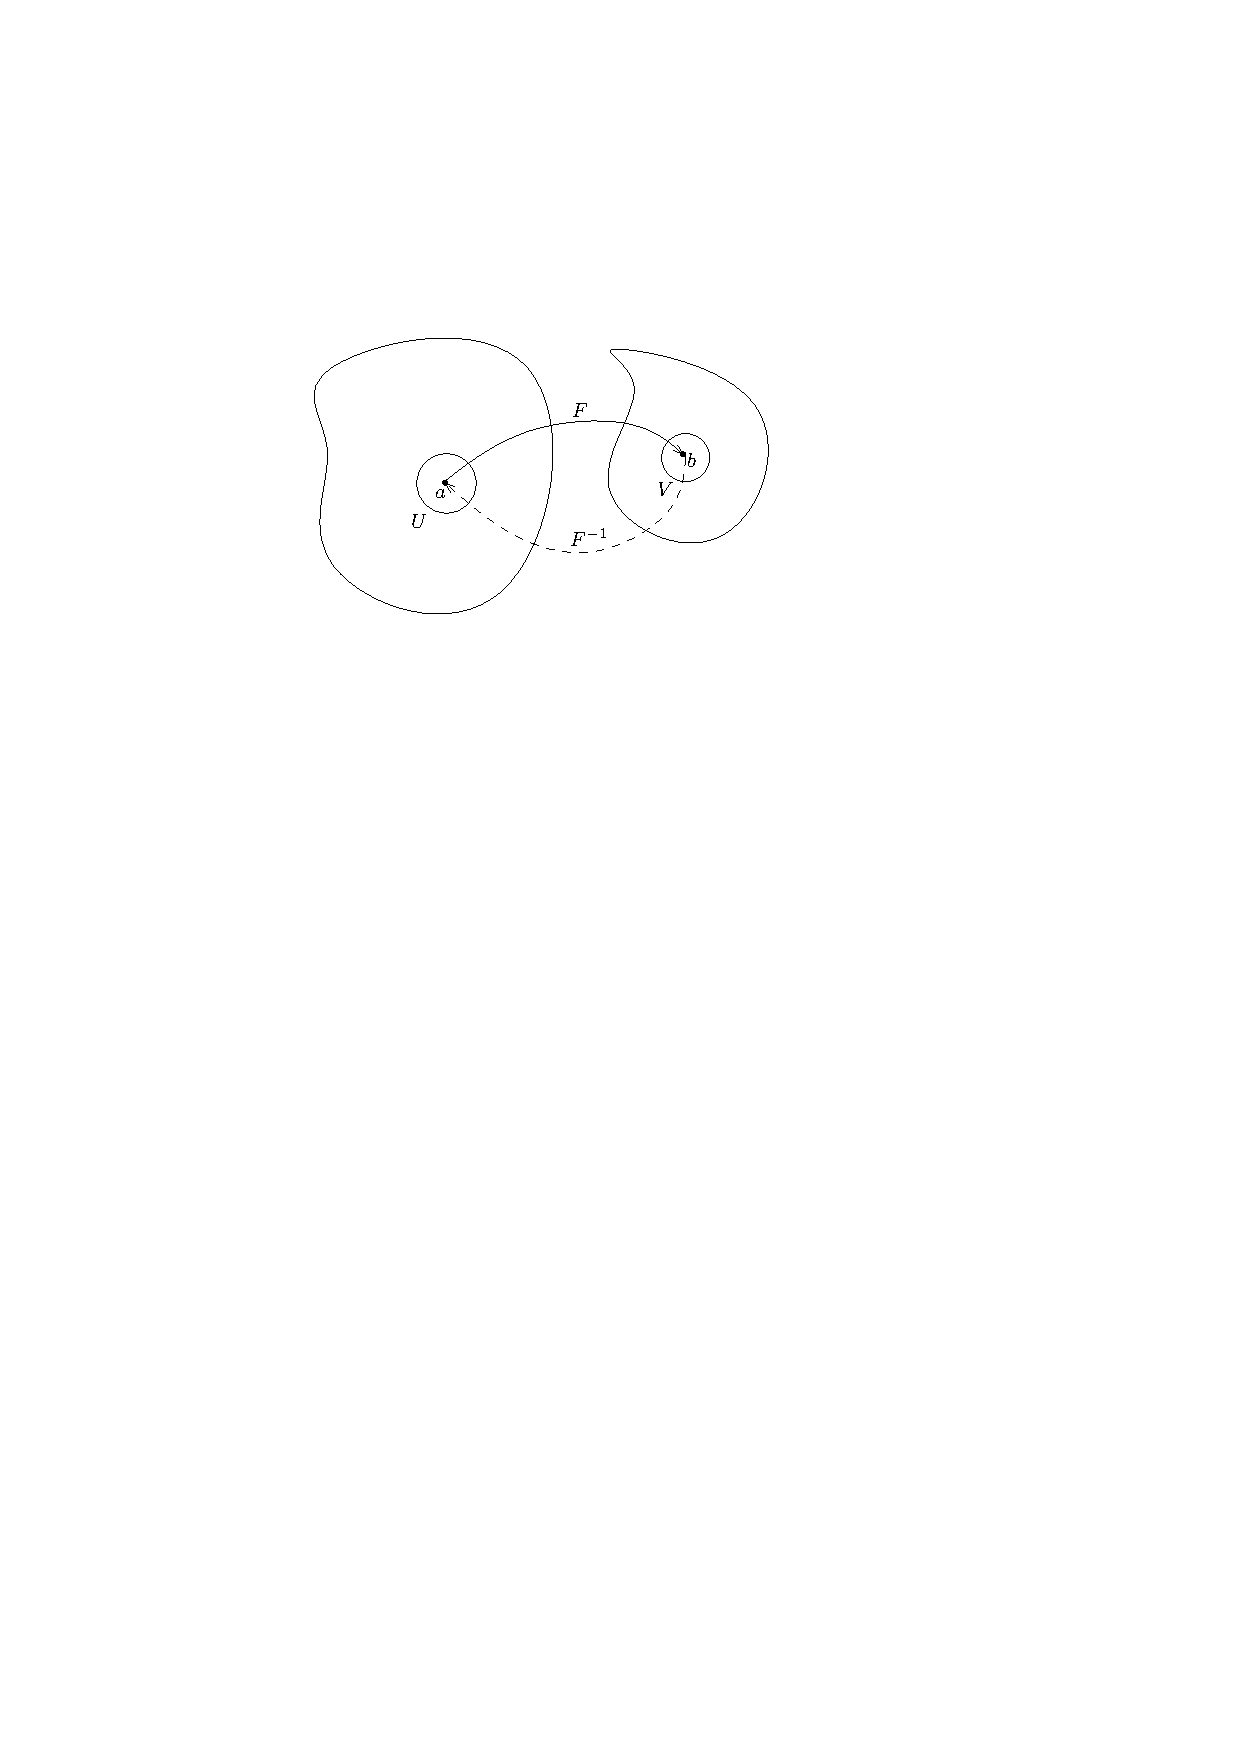
\includegraphics[width=0.6\linewidth]{inversemap}
\end{figure}

\begin{align}
  \Delta F &= F(x) - F(a) = y - b = \Delta y \label{eq:diffspace::invmaphandwave::delta}\\
  \Delta F &= F'(a) dx + o(dx) \\
  \del F(a) &= \del y(b) \label{eq:diffspace::invmaphandwave::diff}
\end{align}

Условие разрешимости \ref{eq:diffspace::invmaphandwave::diff}~--- $\det\bigl(F'(a)\bigr) \neq 0$.
Утверждается, что \ref{eq:diffspace::invmaphandwave::diff} $\Rightarrow$
\ref{eq:diffspace::invmaphandwave::delta}

Соответственно, формулировка 
\begin{thrm}\label{thrm:diffspace::invmaphandwave}
  Пусть $F\colon G\subset \R^n \to \R^n$, $a\in G$, $b = F(a)$. Пусть ещё $F \in C^1$, 
  $\det(F'(a)) \neq 0$
  
  Тогда 
  \[
    \begin{split}
      & \exists\, U(a), V(b) \,\colon\; F \colon U \leftrightarrow V \\
      & \exists\, F^{-1} V\to U, \; F^{-1} \in C^1
    \end{split}
  \]
\end{thrm}

\paragraph{Доказательство теоремы об обратимости}
\label{par:diffspace::invmapproof}

\begin{ittproof}[Теорема об обратимости отображения]
  Введём обозначения:
  \begin{align*}
    F'(a) &= \Gamma\\
    \Phi(x) &= x - \Gamma^{-1} (F(x) - y)
  \end{align*}
  Нетрудно заметить, что $x$~--- неподвижная точка $\Phi$ (что $\Leftrightarrow F(x)=y$ ).
  Очень хотелось бы подогнать всё под теорему Банаха (\ref{thrm:diffspace::contrmap::banach}).
  Тогда отображение в окрестности $a$ будет взаимно-однозначным.

  \begin{enumerate}
    \item Сначала оценим $\|\Phi'\|$.
      \[
        \Phi'(x) = E - \Gamma^{-1} (F'(x)) = \Gamma^{-1} (F'(a) - F'(x))
      \]
      Можно норму оценить
      \[
        \|\Phi'(x)\| = \| \Gamma^{-1} \| \cdot \| (F'(a) - F'(x)) \|
      \]
      Последний множитель явно $\xrightarrow[x\to a]{} 0$ (так как $F\in C^1$)
      Тогда и $\|\Phi'(x)\|\to 0$. А значит найдётся $U_\varepsilon(a) \colon 
      \|\Phi'(x)\| \leqslant \frac{1}{2}$.
      
      Тогда по теореме \ref{thrm:diffspace::diffestim::diffestim} 
      \[
        x, x' \in U_\varepsilon(a) \Rightarrow \| \Phi(x) - \Phi(a)\| \leqslant \frac{1}{2}
        \|x-x'\|
      \]
      Собственно, почти победа. Осталось лишь выбрать внутри $U_\varepsilon$ компакт
      $\overline{U_{\varepsilon_1}}$ (иначе множество не очень полное).

    \item Теперь покажем, что 
      \[
        \exists\, \overline{U} \colon \Phi(U) \subset U  
      \]
      Попутно примем $\|y-b\| < \delta$, это потом поможет доказать непрерывность.
      \[
        \begin{split}
          \|\Phi(x) - a\| = \| x - a - \Gamma^{-1}(F(x)-y)\| 
          \leqslant \|\Gamma^{-1}\| \cdot \| \Gamma (x-a) - F(x) + y + b - b\| \\ 
          \leqslant \|\Gamma^{-1}\| 
          \cdot \bigl(\| - \underbrace{( F(x) - F'(a)(x-a) - F(a) )}_{\alpha}\| + \| y - b\| \bigr)
        \end{split}
      \]
      Выберем произвольный $\varepsilon \colon 0 < \varepsilon < \varepsilon_1$.
      
      Однако мы ещё можем подкрутить $\varepsilon_1$. 
      \[
        \exists\, U_{\varepsilon_1} \colon \frac{\|\alpha\|}{\|x-a\|} < \frac{1}{2\|\Gamma^{-1}\|}
      \]
      Это следует из формулы Тейлора (\ref{thrm:diffspace::taylor}), а применять её можно, так
      как шар~--- выпуклое множество. Ещё выберем $\delta = \frac{\varepsilon}{2\|\Gamma^{-1}\|}$.
      Там правда $\varepsilon$, а не $\varepsilon_1$.

      Тогда цепочка неравенств выше преобразуется к такому виду
      \[
        \ldots < \|\Gamma^{-1}\| \cdot \frac{\|x - a\|}{2\|\Gamma^{-1}\|} +
        \frac{\varepsilon}{2\|\Gamma^{-1}\|} \cdot \|\Gamma^{-1}\|
      \]

      А теперь положим $\|x-a\| \leqslant \varepsilon$ (неравенство нужно нестрогое для полноты). 
      Тогда
      \[
        x\in \overline{U_\varepsilon}(a) \Rightarrow \Phi(x) \in U_{\varepsilon}(a) \subset 
        \overline{U_\varepsilon}(a) 
      \]

      А теперь по теореме Банаха
      \[
        \exists!\, x_0\in \overline{U_\varepsilon}(a) \colon \Phi(x_0) = x_0 \Leftrightarrow
        F(x_0)= y_0 
      \]
      Видимо, осталось пересечь окрестность $a$ с прообразом $V(b)$ : $U = F^{-1}(V) \cap
      U_\varepsilon (a)$
      \item
      Заодно получилась и непрерывность:
      \[
        \forall\, U\; \exists\, V_\delta(b) \colon F^{-1}(V_\delta) \subset
        U_\varepsilon 
      \]
  \end{enumerate}
\end{ittproof}

\paragraph{Теорема о дифференцируемости обратного отображения}
\label{par:diffspace::invdiff}

\begin{thrm}[о дифференцируемости $F^{-1}$]\label{thrm:diffspace::invdiff}
  Пусть $U \subset \R^n$, $V \subset \R^n$, $F\colon U \leftrightarrow V$. Пусть также
  $F$~--- дифференцируемо в $a\in U$, $F(a) = b$,  $\det F'(a) \neq 0$. 
  Тогда $F^{-1}$ дифференцируемо в $b$.
\end{thrm}
\begin{ittproof}
  То, что есть обратное отображение, доказали выше. Пусть $y=F(x)$. Обозначим: $h= x-a$, $k=y-b$.
  Отображение биективно, значит $h\neq 0 \Leftrightarrow k \neq 0$.
  Из дифференцирумости $F$
  \[
    k = y - b = F(x) - F(a) = A h + \alpha \\
    \alpha = o(h) \; (h\to 0)
  \]
  $A = F'(a) \neq 0$, следовательно $\exists\, A^{-1}$
  \[
    A^{-1} k = A^{-1}Ah + A^{-1}\alpha \Rightarrow \Delta F^{-1} = h = A^{-1} k - A^{-1} \alpha
  \]
  Докажем, что $-A^{-1} \alpha =: \beta = o(k) \; (k\to 0) $
  \[
    \beta \leqslant \frac{-\alpha}{\|k\|} = \frac{-\alpha}{\|h\|}\cdot \frac{\|h\|}{\|k\|}  
  \]
  Покажем, что последнй член~--- ограничен
  \[
    \frac{\|h\|}{\|k\|} = \frac{\|h\|}{\|A h + \alpha\|} 
    \leqslant \frac{\|h\|}{\big|\|Ah\|- \|\alpha\|\big|}
    = \frac{1}{\big|\frac{\|Ah\|}{\|h\|} - \frac{\|\alpha\|}{\|h\|}\big|}  
  \]
  А последнее выражение ограничено при $\|h\| < \delta$

\end{ittproof}

\begin{cor*}
  $\displaystyle (F^{-1})'(b) = \bigl(F'(a)\bigr)^{-1}$
\end{cor*}

\paragraph{Теорема о гладкости обратного отображения}
\label{par:diffspace::invsmooth}

\begin{thrm}\label{thrm:diffspace::invsmooth}
  Пусть $F\colon U \leftrightarrow V$, биективна, $\in C^p$. Пусть к тому же $\det F'(x) \neq 0$.
  Тогда $F^{-1} \in C^p$
\end{thrm}
\begin{ittproof}
  Введём обозначения (оно всё существует по предыдущим теоремам хоть где-то)
  \[
    \begin{aligned}
      F'(x) &= \left(\frac{\partial F_i}{\partial x_j}\right)_{i,j=1}^n & &= (a_{ij}) = A \\
      (F^{-1})'(y) &= \left(\frac{\partial F^{-1}_i}{\partial y_j}\right)_{i,j=1}^n & &= (b_{ij}) = B 
    \end{aligned}
  \]
  Вполне ясно, что $B = A^{-1}$. Из алгебры $b_{ij} = \dfrac{\mathcal A_{ji}}{\det A}$ 
  (здесь $\mathcal A$~--- алгебраическое дополнение).
  
  Заметим, что из последнего выражения следует, что $b_{ij}$~--- рациональная функция от $\{a_{lk}\}$.
  Следовательно, $\widetilde{b_{ij}} = b_{ij}(a_{11}, \dotsc, a_{kl}, \dotsc, a_{nn}) \in C^\infty$.
  С другой стороны
  \[
    b_{ij}(y) = \frac{\partial F^{-1}}{\partial y_j}(y) = \frac{\partial F^{-1}}{\partial y_j}\bigl(F(x)\bigr)
    \Leftrightarrow b_{ij}(y) = \widehat{b_{ij}}(x)
  \]

  Так что $\widehat{b_{ij}} = b_{ij} \circ F$. 

  Дальше немного магии. Введём ещё одну функцию
  \[
    \overline{b_{ij}}(x) = b_{ij}(a_{11}(x), \dotsc, a{kl}(x), \dotsc, a_{nn}(x))   
  \]
  Заметим, что каждая $a_{ij}(x) \in C^{p-1} \Rightarrow \overline{b_{ij}} \in C^{p-1}$.
  Хорошо, тогда 
  \[
    b_{ij}(y) = \bigl(\overline{b_{ij}} \circ F^{(-1)}\bigr)(y) 
  \]
  Раньше доказали, что $F^{-1} \in C^0$. Теперь разматываем цепочку дальше:
  \[
    F^{-1} \in C^i \Rightarrow \overline{b_{ij}} \circ F^{-1} \in C^i \Rightarrow b_{ij} \in C^i 
  \]
  Значит, частные производные $F^{-1}$ принадлежат $C^i$. Тогда сама $F^{-1} \in C^{i+1}$.
  Таким бобром мы доберёмся до $C^p$. 
  Дальше не выйдет, так как не хватит гладкости $\overline{b_{ij}}$.
\end{ittproof}

\paragraph{Гладкая зависимость корней многочлена от его коэффициентов}
\label{par:diffspace::smoothpolyroots}

\begin{thrm}\label{thrm:diffspace::smoothpolyroots}
  Пусть $P(x) \in \R[x]$ имеет $n$ корней $(x^0_j)$,  $x^0_j \in \R$, таких что $\forall\, i,j \; x^0_i \neq x^0_j$.  
  Тогда 
  \[
    x_i = x_i(a_0, \dotsc, a_{n-1}) \in C^\infty
  \]
\end{thrm}

\begin{ittproof}
  Пусть $P(x) = (x - x_1) \dotsm (x - x_n)$. Вспомним теорему Виета (из алгебры)
  \begin{align*}
    a_0     & = (-1)^n x_1 \dotsm x_n \\
    a_1     & = (-1)^{n-1} \sum_{i} \prod_{j \neq i} x_j \\
            & \cdots \cdots \cdots  \\
    a_{n-1} & = (-1) \sum_i x_i
  \end{align*}

  Рассмотрим $P$ как отображение $(x_1, \dotsc, x_n) \mapsto (a_0, \dotsc, a_{n-1})$.
  \[
    P'(x) = 
    \begin{pmatrix}
      \frac{\partial P_1}{\partial x_1} & \cdots & \frac{\partial P_1}{\partial x_n} \\
      \vdots & \ddots & \vdots \\
      \frac{\partial P_n}{\partial x_1} & \cdots & \frac{\partial P_n}{\partial x_n} \\
    \end{pmatrix}
    = 
    \begin{pmatrix}
      (-1)^n \prod_{i\neq 1} x_i & (-1)^n \prod_{i\neq 2} x_i & \cdots & (-1)^n \prod_{i\neq n} x_i \\
      \hdotsfor{4} \\
      -1 & -1 & \cdots & -1 
    \end{pmatrix}
  \]
  Посчитаем $\det(F')$. Этот определитель можно рассмотреть как многочлен $\in R[x_1, \dotsc, x_n]$
  Его степень не превосходит $0 + 1 + \dotsb + (n-1) = \frac{n(n-1)}{2}$. Заметим, что если хоть
  какая-то пара столбиков равны, то определитель равен нулю. Так что $\det(F')$ делится на
  всевозможные многочлены вида $x_i - x_j$. А их как раз $\frac{n(n-1)}{2}$ и они неприводимые.
  Следовательно, 
  \[
    \det (F')(x_1, \dotsc, x_n) = C \prod_{i<j} (x_i - x_j) 
  \]
  А значит при условии неравенства корней он ненулевой.
  \footnote{Этого, конечно не было в курсе алгебры, но там не используется ничего страшнее
  теоремы о делении с остатком. Вообще доказать бы надо, но лень.}

  Дальше можно воспользоваться теоремой о гладкости обратного отображения.
\end{ittproof}

\paragraph{Теорема о неявном отображении}
\label{par:diffspace::implicit}



\end{document}
